% questions.tex —— 2001 年·全国旧课程卷·理科 · 题目内容片段（无答案）
% 由 tools/generate_projects.py 依来源总账自 2001/2001_数学真题_全国旧课程理_试题.md 生成，勿手改（改源 MD 后重跑）


\gkpart{理科数学}

\begin{gktip}
\textbf{来源说明}：本题面依据固定源 PDF《2001 普通高等学校招生考试（全国卷理）》逐题转录。固定源为 2 页 A3 横向题面，原卷印刷页码 85–86；PDF 不含答案或解析页，下列答案和解析由本库独立推导，不声称代表官方发布版本。

\textbf{图形说明}：第 5、11、12、17 题的原卷图形关系重绘为 TikZ/PGFPlots 矢量图。图形标记所指的 PNG 不随仓库保存。
\end{gktip}

\gkpart{一、选择题}

\begin{question}
\gkti{1}若 $\sin\theta\cos\theta>0$，则 $\theta$ 在\mbox{（　　）}

（A）第一、二象限　　（B）第一、三象限　　（C）第一、四象限　　（D）第二、四象限

\end{question}
\begin{question}
\gkti{2}过点 $A(1,-1)$、$B(-1,1)$ 且圆心在直线 $x+y-2=0$ 上的圆的方程是\mbox{（　　）}

（A）$(x-3)^2+(y+1)^2=4$　　（B）$(x+3)^2+(y-1)^2=4$

（C）$(x-1)^2+(y-1)^2=4$　　（D）$(x+1)^2+(y+1)^2=4$

\end{question}
\begin{question}
\gkti{3}设 $\{a_n\}$ 是递增等差数列，前三项的和为 $12$，前三项的积为 $48$，则它的首项是\mbox{（　　）}

（A）$1$　　（B）$2$　　（C）$4$　　（D）$6$

\end{question}
\begin{question}
\gkti{4}若定义在区间 $(-1,0)$ 内的函数 $f(x)=\log_{2a}(x+1)$ 满足 $f(x)>0$，则 $a$ 的取值范围是\mbox{（　　）}

（A）$\left(0,\dfrac12\right)$　　（B）$\left(0,\dfrac12\right]$　　（C）$\left(\dfrac12,+\infty\right)$　　（D）$(0,+\infty)$

\Needspace{0.4\textheight}
\end{question}
\begin{question}
\gkti{5}极坐标方程 $\rho=2\sin\left(\theta+\dfrac\pi4\right)$ 的图形是\mbox{（　　）}
\nopagebreak[4]
\begin{center}% 2001 年全国旧课程卷理科第 5 题：极坐标方程的四个图象选项
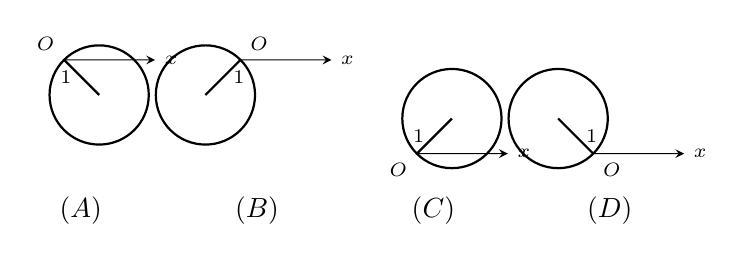
\begin{tikzpicture}[>=stealth, scale=0.70]
  \begin{scope}
    \coordinate (O) at (0,0.85);
    \coordinate (C) at (0.636,0.214);
    \draw[thick] (C) circle (0.9);
    \draw[thick] (O)--(C) node[midway, left, font=\scriptsize] {$1$};
    \draw[->] (O)--(1.65,0.85) node[right, font=\scriptsize] {$x$};
    \node[above left, font=\scriptsize] at (O) {$O$};
    \node[below] at (0.3,-1.45) {$(A)$};
  \end{scope}
  \begin{scope}[xshift=3.2cm]
    \coordinate (O) at (0,0.85);
    \coordinate (C) at (-0.636,0.214);
    \draw[thick] (C) circle (0.9);
    \draw[thick] (O)--(C) node[midway, right, font=\scriptsize] {$1$};
    \draw[->] (O)--(1.65,0.85) node[right, font=\scriptsize] {$x$};
    \node[above right, font=\scriptsize] at (O) {$O$};
    \node[below] at (0.3,-1.45) {$(B)$};
  \end{scope}
  \begin{scope}[xshift=6.4cm]
    \coordinate (O) at (0,-0.85);
    \coordinate (C) at (0.636,-0.214);
    \draw[thick] (C) circle (0.9);
    \draw[thick] (O)--(C) node[midway, left, font=\scriptsize] {$1$};
    \draw[->] (O)--(1.65,-0.85) node[right, font=\scriptsize] {$x$};
    \node[below left, font=\scriptsize] at (O) {$O$};
    \node[below] at (0.3,-1.45) {$(C)$};
  \end{scope}
  \begin{scope}[xshift=9.6cm]
    \coordinate (O) at (0,-0.85);
    \coordinate (C) at (-0.636,-0.214);
    \draw[thick] (C) circle (0.9);
    \draw[thick] (O)--(C) node[midway, right, font=\scriptsize] {$1$};
    \draw[->] (O)--(1.65,-0.85) node[right, font=\scriptsize] {$x$};
    \node[below right, font=\scriptsize] at (O) {$O$};
    \node[below] at (0.3,-1.45) {$(D)$};
  \end{scope}
\end{tikzpicture}
\end{center}
\nopagebreak[4]
\end{question}
\begin{question}
\gkti{6}函数 $y=\cos x+1\ (-\pi\le x\le0)$ 的反函数是\mbox{（　　）}

（A）$y=-\arccos(x-1)\ (0\le x\le2)$

（B）$y=\pi-\arccos(x-1)\ (0\le x\le2)$

（C）$y=\arccos(x-1)\ (0\le x\le2)$

（D）$y=\pi+\arccos(x-1)\ (0\le x\le2)$

\end{question}
\begin{question}
\gkti{7}若椭圆经过原点，且焦点为 $F_1(1,0)$、$F_2(3,0)$，则其离心率为\mbox{（　　）}

（A）$\dfrac34$　　（B）$\dfrac23$　　（C）$\dfrac12$　　（D）$\dfrac14$

\end{question}
\begin{question}
\gkti{8}若 $0<\alpha<\beta<\dfrac\pi4$，$\sin\alpha+\cos\alpha=a$，$\sin\beta+\cos\beta=b$，则\mbox{（　　）}

（A）$a>b$　　（B）$a<b$　　（C）$ab<1$　　（D）$ab>2$

\end{question}
\begin{question}
\gkti{9}在正三棱柱 $ABC-A_1B_1C_1$ 中，若 $AB=\sqrt2BB_1$，则 $AB_1$ 与 $C_1B$ 所成的角的大小为\mbox{（　　）}

（A）$60^\circ$　　（B）$90^\circ$　　（C）$45^\circ$　　（D）$120^\circ$

\end{question}
\begin{question}
\gkti{10}设 $f(x)$、$g(x)$ 都是单调函数，有如下四个命题中，正确的命题是\mbox{（　　）}

① 若 $f(x)$ 单调递增，$g(x)$ 单调递增，则 $f(x)-g(x)$ 单调递增；

② 若 $f(x)$ 单调递增，$g(x)$ 单调递减，则 $f(x)-g(x)$ 单调递增；

③ 若 $f(x)$ 单调递减，$g(x)$ 单调递增，则 $f(x)-g(x)$ 单调递减；

④ 若 $f(x)$ 单调递减，$g(x)$ 单调递减，则 $f(x)-g(x)$ 单调递减。

（A）①③　　（B）①④　　（C）②③　　（D）②④

\Needspace{0.4\textheight}
\end{question}
\begin{question}
\gkti{11}一间民房的屋顶有如图三种不同的盖法：① 单向倾斜；② 双向倾斜；③ 四向倾斜。记三种盖法屋顶面积分别为 $P_1$、$P_2$、$P_3$。若屋顶斜面与水平面所成的角都是 $\alpha$，则\mbox{（　　）}
\nopagebreak[4]
\begin{center}% 2001 年全国旧课程卷理科第 11 题：三种屋顶盖法
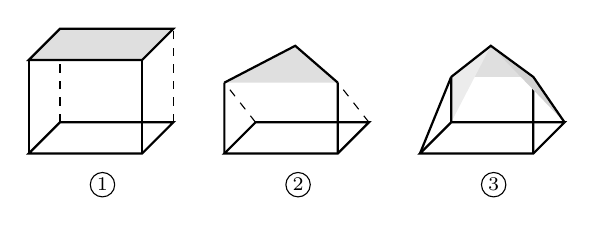
\begin{tikzpicture}[>=stealth, scale=0.72]
  \begin{scope}
    \coordinate (A) at (0,0);
    \coordinate (B) at (2.0,0);
    \coordinate (C) at (2.55,0.55);
    \coordinate (D) at (0.55,0.55);
    \coordinate (A1) at (0,1.65);
    \coordinate (B1) at (2.0,1.65);
    \coordinate (C1) at (2.55,2.2);
    \coordinate (D1) at (0.55,2.2);
    \draw[thick] (A)--(B)--(C)--(D)--cycle;
    \draw[thick] (A)--(A1) (B)--(B1);
    \draw[dashed] (C)--(C1) (D)--(D1);
    \fill[gray!25] (A1)--(B1)--(C1)--(D1)--cycle;
    \draw[thick] (A1)--(B1)--(C1)--(D1)--cycle;
    \node[circle,draw,inner sep=1pt] at (1.3,-0.55) {\scriptsize 1};
  \end{scope}
  \begin{scope}[xshift=3.45cm]
    \coordinate (A) at (0,0);
    \coordinate (B) at (2.0,0);
    \coordinate (C) at (2.55,0.55);
    \coordinate (D) at (0.55,0.55);
    \coordinate (M) at (1.25,1.9);
    \draw[thick] (A)--(B)--(C)--(D)--cycle;
    \draw[thick] (A)--(0,1.25) (B)--(2,1.25);
    \draw[dashed] (C)--(2,1.25) (D)--(0,1.25);
    \fill[gray!25] (0,1.25)--(M)--(2,1.25)--cycle;
    \draw[thick] (0,1.25)--(M)--(2,1.25);
    \node[circle,draw,inner sep=1pt] at (1.3,-0.55) {\scriptsize 2};
  \end{scope}
  \begin{scope}[xshift=6.9cm]
    \coordinate (A) at (0,0);
    \coordinate (B) at (2.0,0);
    \coordinate (C) at (2.55,0.55);
    \coordinate (D) at (0.55,0.55);
    \coordinate (M) at (1.25,1.9);
    \coordinate (L) at (0.55,1.35);
    \coordinate (R) at (2.0,1.35);
    \draw[thick] (A)--(B)--(C)--(D)--cycle;
    \draw[thick] (A)--(L) (B)--(R);
    \draw[dashed] (C)--(R) (D)--(L);
    \fill[gray!25] (L)--(M)--(R)--cycle;
    \fill[gray!15] (D)--(L)--(M)--cycle;
    \fill[gray!35] (M)--(R)--(C)--cycle;
    \draw[thick] (L)--(M)--(R) (D)--(L) (R)--(C);
    \node[circle,draw,inner sep=1pt] at (1.3,-0.55) {\scriptsize 3};
  \end{scope}
\end{tikzpicture}
\end{center}
\nopagebreak[4]
（A）$P_3>P_2>P_1$　　（B）$P_3>P_2=P_1$　　（C）$P_3=P_2>P_1$　　（D）$P_3=P_2=P_1$

\Needspace{0.4\textheight}
\end{question}
\begin{question}
\gkti{12}如图，小圆圈表示网络的结点，结点之间的连线表示它们有网线相联。连线标注的数字表示该段网线单位时间内可以通过的最大信息量。现从结点 $A$ 向结点 $B$ 传递信息，信息可以分开沿不同的路线同时传递，则单位时间内传递的最大信息量为\mbox{（　　）}
\nopagebreak[4]
\begin{center}% 2001 年全国旧课程卷理科第 12 题：信息网络
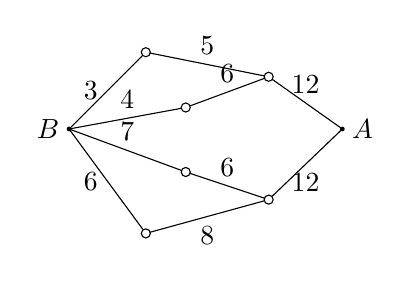
\begin{tikzpicture}[>=stealth, scale=0.78]
  \coordinate (B) at (0,0);
  \coordinate (U) at (1.25,1.25);
  \coordinate (V) at (3.25,0.85);
  \coordinate (M) at (1.9,0.35);
  \coordinate (N) at (1.9,-0.7);
  \coordinate (W) at (1.25,-1.7);
  \coordinate (Z) at (3.25,-1.15);
  \coordinate (A) at (4.45,0);

  \draw (B)--(U) node[midway, left] {3};
  \draw (U)--(V) node[midway, above] {5};
  \draw (B)--(M) node[midway, above] {4};
  \draw (M)--(V) node[midway, above] {6};
  \draw (B)--(N) node[midway, above] {7};
  \draw (N)--(Z) node[midway, above] {6};
  \draw (B)--(W) node[midway, left] {6};
  \draw (W)--(Z) node[midway, below] {8};
  \draw (V)--(A) node[midway, above] {12};
  \draw (Z)--(A) node[midway, below] {12};

  \foreach \point in {U,V,M,N,W,Z}
    \filldraw[fill=white] (\point) circle (2.1pt);
  \fill (B) circle (1.1pt) node[left] {$B$};
  \fill (A) circle (1.1pt) node[right] {$A$};
\end{tikzpicture}
\end{center}
\nopagebreak[4]
（A）$26$　　（B）$24$　　（C）$20$　　（D）$19$

\end{question}
\gkpart{二、填空题}

\begin{question}
\gkti{13}若一个圆锥的轴截面是等边三角形，其面积为 $\sqrt3$，则这个圆锥的侧面积是\gkblank{}。

\end{question}
\begin{question}
\gkti{14}双曲线 $\dfrac{x^2}{9}-\dfrac{y^2}{16}=1$ 的两个焦点为 $F_1,F_2$，点 $P$ 在双曲线上，若 $PF_1\perp PF_2$，则点 $P$ 到 $x$ 轴的距离为\gkblank{}。

\end{question}
\begin{question}
\gkti{15}设 $\{a_n\}$ 是公比为 $q$ 的等比数列，$S_n$ 是它的前 $n$ 项和。若 $\{S_n\}$ 是等差数列，则 $q=$\gkblank{}。

\end{question}
\begin{question}
\gkti{16}圆周上有 $2n$ 个等分点（$n>1$），以其中三个点为顶点的直角三角形的个数为\gkblank{}。

\end{question}
\gkpart{三、解答题}

\Needspace{0.4\textheight}
\begin{question}
\gkti{17}如图，在底面是直角梯形的四棱锥 $S-ABCD$ 中，$\angle ABC=90^\circ$，$SA\perp$ 面 $ABCD$，$SA=AB=BC=1$，$AD=\dfrac12$。
\nopagebreak[4]
\begin{center}% 2001 年全国旧课程卷理科第 17 题：直角梯形底面的四棱锥
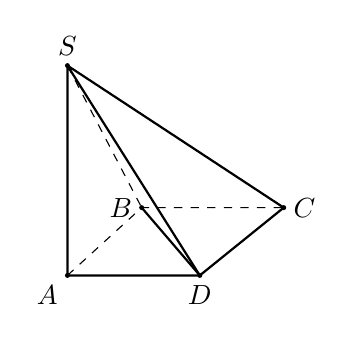
\begin{tikzpicture}[>=stealth, scale=0.82]
  \coordinate (A) at (0,0);
  \coordinate (B) at (1.15,1.05);
  \coordinate (C) at (3.35,1.05);
  \coordinate (D) at (2.05,0);
  \coordinate (S) at (0,3.25);

  \draw[thick] (S)--(A) (S)--(C) (S)--(D);
  \draw[dashed] (S)--(B);
  \draw[thick] (A)--(D)--(C);
  \draw[dashed] (A)--(B)--(C);
  \draw[thick] (B)--(D);

  \fill (S) circle (1.1pt) node[above] {$S$};
  \fill (A) circle (1.1pt) node[below left] {$A$};
  \fill (B) circle (1.1pt) node[left] {$B$};
  \fill (C) circle (1.1pt) node[right] {$C$};
  \fill (D) circle (1.1pt) node[below] {$D$};
\end{tikzpicture}
\end{center}
\nopagebreak[4]
（1） 求四棱锥 $S-ABCD$ 的体积；

（2） 求面 $SCD$ 与面 $SBA$ 所成的二面角的正切值。

\end{question}
\begin{question}
\gkti{18}已知复数 $z_1=i(1-i)^3$。

（1） 求 $\arg z_1$ 及 $|z_1|$；

（2） 当复数 $z$ 满足 $|z|=1$，求 $|z-z_1|$ 的最大值。

\end{question}
\begin{question}
\gkti{19}设抛物线 $y^2=2px\ (p>0)$ 的焦点为 $F$，经过点 $F$ 的直线交抛物线于 $A$、$B$ 两点。点 $C$ 在抛物线的准线上，且 $BC\parallel x$ 轴。证明直线 $AC$ 经过原点 $O$。

\end{question}
\begin{question}
\gkti{20}已知 $i,m,n$ 是正整数，且 $1<i\le m<n$。

（1） 证明：$n^iA_m^i<m^iA_n^i$；

（2） 证明：$(1+m)^n>(1+n)^m$。

\end{question}
\begin{question}
\gkti{21}从社会效益和经济效益出发，某地投入资金进行生态环境建设，并以此发展旅游产业。根据规划，本年度投入 $800$ 万元，以后每年投入将比上年减少 $\dfrac15$。本年度当地旅游业收入估计为 $400$ 万元，由于该项建设对旅游业的促进作用，预计今后的旅游业收入每年会比上年增加 $\dfrac14$。

（1） 设 $n$ 年内（本年度为第一年）总投入为 $a_n$ 万元，旅游业总收入为 $b_n$ 万元。写出 $a_n$、$b_n$ 的表达式；

（2） 至少经过几年旅游业的总收入才能超过总投入？

\end{question}
\begin{question}
\gkti{22}设 $f(x)$ 是定义在 $\mathbb R$ 上的偶函数，其图象关于直线 $x=1$ 对称。对任意 $x_1,x_2\in\left[0,\dfrac12\right]$，都有 $f(x_1+x_2)=f(x_1)\cdot f(x_2)$，且 $f(1)=a>0$。

（1） 求 $f\left(\dfrac12\right),f\left(\dfrac14\right)$；

（2） 证明：$f(x)$ 是周期函数；

（3） 记 $a_n=f\left(2n+\dfrac1{2n}\right)$，求 $\displaystyle\lim_{n\to\infty}\ln a_n$。

\end{question}